\documentclass[13pt,a4paper]{article}
\usepackage[spanish,es-nodecimaldot]{babel}	% Utilizar español
\usepackage[utf8]{inputenc}					% Caracteres UTF-8
\usepackage{graphicx}						% Imagenes
\usepackage[hidelinks]{hyperref}			% Poner enlaces sin marcarlos en rojo
\usepackage{fancyhdr}						% Modificar encabezados y pies de pagina
\usepackage{float}							% Insertar figuras
\usepackage[textwidth=390pt]{geometry}		% Anchura de la pagina
\usepackage[nottoc]{tocbibind}				% Referencias (no incluir num pagina indice en Indice)
\usepackage{enumitem}						% Permitir enumerate con distintos simbolos
\usepackage[T1]{fontenc}					% Usar textsc en sections
\usepackage{amsmath}						% Símbolos matemáticos
\usepackage[ruled,vlined]{algorithm2e}      % Pseudocódigo
\usepackage{xcolor}
\usepackage{listings}
% Para que acepten tíldes los listing
\lstset{     
     literate=%
         {á}{{\'a}}1
         {é}{{\'e}}1
         {í}{{\'i}}1
         {ó}{{\'o}}1
         {ú}{{\'u}}1
         {Á}{{\'A}}1
         {É}{{\'E}}1
         {Í}{{\'I}}1
         {Ó}{{\'O}}1 
         {Ú}{{\'U}}1
         {ñ}{{\~n}}1 
         {Ñ}{{\~N}}1 
         {¿}{{?``}}1 
         {¡}{{!``}}1
}
\usepackage{dsfont}

% ==============================================================================

\usepackage{caption, subcaption}
\usepackage[section]{placeins}
\makeatletter
\def\fps@figure{H}
\makeatother

\usepackage{booktabs}
\usepackage{longtable}
\usepackage{array}
\usepackage{multirow}
\usepackage{wrapfig}
\usepackage{colortbl}
\usepackage{pdflscape}
\usepackage{tabu}
\usepackage{threeparttable}
\usepackage{threeparttablex}
\usepackage[normalem]{ulem}
\usepackage{makecell}
\usepackage{xcolor}
\usepackage[bottom]{footmisc}

\makeatletter
\newcommand*{\centerfloat}{%
  \parindent \z@
  \leftskip \z@ \@plus 1fil \@minus \textwidth
  \rightskip\leftskip
  \parfillskip \z@skip}
\makeatother

% ==============================================================================
% ==============================================================================

% Comando para poner el nombre de la asignatura
\newcommand{\asignatura}{Emprendimiento y transferencia del conocimiento}
\newcommand{\autor}{Ignacio Vellido Expósito}
\newcommand{\email}{ignaciove@correo.ugr.es}
\newcommand{\titulo}{Trabajos}
\newcommand{\subtitulo}{Manejo de rutas y localización de aseos}

% Configuracion de encabezados y pies de pagina
\pagestyle{fancy}
\lhead{\autor{}}
\rhead{\asignatura{}}
\lfoot{Máster Ciencia de Datos e Ingeniería de Computadores}
\cfoot{}
\rfoot{\thepage}
\renewcommand{\headrulewidth}{0.4pt}		% Linea cabeza de pagina
\renewcommand{\footrulewidth}{0.4pt}		% Linea pie de pagina

% ==============================================================================
% ==============================================================================

\begin{document}
    \pagenumbering{gobble}
    % ==============================================================================
% Pagina de titulo
\begin{titlepage}
    \begin{minipage}{\textwidth}
        \centering

        
\includegraphics[scale=0.5]{img/ugr.png}\\

        \textsc{\Large \asignatura{}\\[0.2cm]}
        \textsc{MÁSTER CIENCIA DE DATOS E INGENIERÍA DE COMPUTADORES}\\[1cm]

        \noindent\rule[-1ex]{\textwidth}{1pt}\\[1.5ex]
        \textsc{{\Huge \titulo\\[0.5ex]}}
        \textsc{{\Large \subtitulo\\}}
        \noindent\rule[-1ex]{\textwidth}{2pt}\\[2.5ex]

        \end{minipage}

        \vspace{0.3cm}

        \begin{minipage}{\textwidth}

        \centering

        \textbf{Autor}\\ {\autor{} \\ ignaciove@correo.ugr.es}\\[1.5ex]
        \vspace{0.4cm}

        
\includegraphics[scale=0.3]{img/etsiit.jpeg}
        
\includegraphics[scale=0.6]{img/master.png}

        \vspace{0.7cm}
        \textsc{Escuela Técnica Superior de Ingenierías Informática y de Telecomunicación}\\
        \vspace{1cm}
        \textsc{Curso 2020-2021}
    \end{minipage}
\end{titlepage}
% ==============================================================================
    
    \pagenumbering{arabic}
    \tableofcontents
    \thispagestyle{empty}				% No usar estilo en la pagina de indice

    \newpage

    % ==============================================================================

    % •    Desarrollo de una propuesta sencilla de plan inicial (modelo de negocio) utilizando el método CANVAS + DAFO.
    % •    Realización de una ficha de búsqueda de financiación empresarial.
    % •    Ejercicio práctico de búsqueda de patentes.
    % •    Realización en casa de un video individual (“Elevator Pitch” de menos de 5 minutos) grabado por cada estudiante, presentando su idea de negocio.
    % •    Realización de una tabla con previsiones financieras
    % •    Ejercicio de desarrollo de creatividad y de liderazgo.

    % \section{Modelo CANVAS}

% Aquí una imagen

% 9 campos del canvas y explicarlos

% Canvas (esquema y describirlo, en presentación quizás)

\subsection{Segmento de clientes}

% SC-­‐ Segmento de clientes: grupos de personas o entidades a las que dirigimos las propuestas de valor. ¿Para quien creamos valor? ¿Nos dirigimos a uno o a diferentes segmentos? (Mercado de masas, nicho de mercado, mercado segmentado) . 

La app se puede dirigir a cualquier grupo de personas que posean un móvil, pero debemos tener en cuenta que el problema que pretende resolver puede ser vergonzoso o ridículo para gran parte de la población.

Por tanto, debemos enfocarnos en diferentes tipos de público objetivo que permitan (volver normal) y arrancar el negocio. Estos son:
\begin{itemize}
    \item \textbf{Turistas}: Estando en una ciudad desconocida y sentir la necesidad puede ser un problema grande. Si con el tiempo es posible alcanzar un rango de efectividad semi-global este sector podrá ser muy prometedor.
    \item \textbf{Trabajadores en la calle}: En este sector englobamos personas tales como taxistas, transportistas (camioneros), y cualquier tipo de persona que se desplace constantemente en sus horarios de trabajo. La probabilidad de uso de la aplicación por parte de este grupo de usuarios es menor pues gran parte de ellos ya conocerán lugares donde ir al servicio. Aunque nuestra app probablemente tengo un uso más esporádico, la inclusión de estimación de ocupación e higiene puede ser útil para este grupo de personas.
    \item \textbf{Usuarios con problemas intestinales}: Principal público objetivo. Al ser conscientes de su enfermedad tendrán hábitos y preocupaciones que los inciten a usar la aplicación, con la idea de tener el máximo de información es sus decisiones (por ej: un usuario puede usar la información para decidir dónde comer si cree que va a tener una urgencia tras la comida).
\end{itemize}

\subsection{Propuesta de valor}

% PV-­‐ Propuestas de valor: productos y servicios que crean valor para un segmento de mercado específico. El obje8vo es solucionar los problemas de los clientes: “Qué quiere comprar nuestro cliente" versus "qué vendemos". 

Proponemos información detallada y a tiempo real de los mejores lugares en los que ir al baño para nuestros usuarios. Para tenemos en cuenta no solo las preferencias del cliente (nivel de urgencia, localización) sino también la calidad de los posibles lugares (higiene, ocupación).

Todo esto además se ofrece de manera gratuita para el usuario.

\subsection{Canales de comunicación, distribución y venta}

% C-­‐ Canales de comunicación, distribución y venta: la forma en que la empresa establece contacto con los diferentes clientes y cómo les proporciona la propuesta de valor. 

% Anuncios en redes sociales, Youtube. Se espera que a la larga la manera que resulte más eficiente sea el boca-a-boca.

% Soporte mediante una página web ?

\subsection{Relación con los clientes}

% RC-­‐ Relación con los clientes: relaciones de la empresa con cada segmento de clientes. En función de cada cliente, adaptaremos el discurso.

\subsection{Ingresos}

% I-­‐Ingresos: se generan cuando los clientes compran las propuestas de valor que ofrece la empresa. ¿Por qué valor pagarían nuestros clientes? ¿Cómo pagan ahora? ¿Cómo les gustaría pagar? 

Se podría considerar añadir información extra tras algunos modelos de pago, pero es esencial que la funcionalidad principal se ofrezca gratuítamente al usuario si queremos alcanzar fidelidad con ellos. Esto nos deja con dos posibles formas de ganar ingresos:

\begin{itemize}
    \item Anuncios de manera no intrusiva, de forma que no empeoremos la opinión de los usuarios.
    \item Venta de datos.
\end{itemize}

\subsection{Recursos y capacidades}

% RC-­‐Recursos y capacidades clave: acFvos necesarios para el modelo de negocio, incluidas las personas de la empresa y sus capacidades (Recursos esicos, intelectuales, humanos, y económicos). 

\begin{itemize}
    \item Servidores y bases de datos que soporten el sistema. Preferiblemente contratado mediante un modelo SaaS.
    \item Personal de desarrollo, soporte, y reparación de la aplicación ante posibles caídas.
    \item Personal legal y de recursos humanos ?
\end{itemize}

\subsection{Actividades clave}

% AC-­‐Ac8vidades clave: acciones necesarias que deben llevarse a cabo si contamos con las capacidades y recursos necesarios (Producción, I+D, Resolución de problemas, Plataforma..) 

\subsection{Partners clave}
% Google y Apple ?

% PC -­‐ Partners (Alianzas) clave: las alianzas, los socios, incluso los proveedores que necesitamos para el éxito del modelo de negocio. Algunas acFvidades se pueden externalizar. 

Se podrían usar mapas de software libre.
En otro caso, si quisiéramos usar las APIs de Google y Apple, deberíamos tener una buena relación con ellos.

\subsection{Estructura de costes}

% EC-­‐ Estructura de costes: gastos asociados a la puesta en marcha de un negocio para poder elaborar y hacer llegar la propuesta de valor a los clientes (Costes fijos, variables, low-­‐cost, según valor, economias de escala,..)

El coste de los recursos tecnológicos tendrá una base fija y una variable en función de la demanda de usuarios y el rango de soporte (países) de la aplicación.
Existe también un coste de distribución en las tiendas de software móvil (App Store y Play Store)

Coste fijo del personal técnico y (legal?) \newpage
    \section{Patentes}

\subsection{}

Buscar patentes de relacionadas con el campo de vuestra idea de negocio (por ejemplo patentes relacionadas con redes neuronales, patentes relacionadas con lógica difusa, etc. Si vuestra idea de negocio o tecnología se relaciona con “soft-computing”). Buscar con palabras clave (key words).

\par\noindent\rule{\textwidth}{0.4pt}

He buscado patentes a partir de las keywords ``robot dog''.

\begin{itemize}
    \item ¿Cuántas son?. Utilizando LENS indicar con un gráfico cómo es la evolución de patentes en este campo.
    
    \begin{itemize}
        \item LENS: 20.846 patentes.
        \item Google patents: 75.624 patentes.
        \item Espacenet: 13.335 patentes.
    \end{itemize}
    
    \begin{figure}[H]
        \centering
        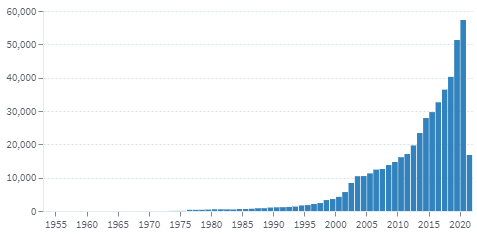
\includegraphics[width=.8\textwidth]{img/patentes/2a.png}
    \end{figure}

    Mirando por encima no todas patentan un robot al completo. Muchas de ellas describen sistemas de visión, sistemas de control, circuitos\dots.

    \item Identificar algún código de clasificación de patentes (CPC o CIP) relacionado.
    
    He visto 2 códigos CPC frecuentemente:
    \begin{itemize}
        \item A63H11/00: Derivado de salud y juguetes.
        \item B25J19/00: Para sistema de control de manipuladores.
    \end{itemize}

    \item Indicar número de patentes de ese código (CPC o CIP).
    \begin{itemize}
        \item A63H11/00: 5.396 patentes.
        \item B25J19/00: 48.745 patentes.
    \end{itemize}

    \item Indicar las tres principales empresas que tienen patentes relacionadas con ese código (CPC o CIP).
    \begin{itemize}
        \item A63H11/00: Sony Corp (636), Mattel INC (172), Groove X INC (95).
        \item B25J19/00: Fanuc LTD (1.164), Seiko Epson Corp (590), Kawasaki Heavy Industries (461).
    \end{itemize}

    \item Buscar una patente en concreto e indicar el link donde aparezcan los “claims” (o reivindicaciones) de una patente en este campo.
    
    Patente CN205273661U:

    \url{https://worldwide.espacenet.com/patent/search/family/056058262/publication/CN205273661U?q=pn%3DCN205273661U}
\end{itemize}


\subsection{}

A la hora de valorar patentes se puede tener en cuenta el crecimiento del área tecnológica, que a su vez se puede medir de forma indirecta analizando el crecimiento registrado en el número de solicitudes de patente en un área específica de la tecnología, valorando positivamente aquellas tecnologías cuyas patentes hayan registrado un crecimiento continuado en el pasado reciente (20 años) frente a las que hayan registrado un crecimiento negativo, discontinuo o alejado en el tiempo.

Buscar tendencias de patentes en las siguientes temáticas (utilizar el buscador “LENS”).

Para cada caso añadir el gráfico de tendencia anual de patentes sobre esta temática (gráfico de número de patentes por año relacionadas con ese campo):

\par\noindent\rule{\textwidth}{0.4pt}

\begin{itemize}
    \item Buscar patentes sobre “Face recognition”. Indicar cuántas tiene “Samsung” sobre esta temática

    498.029 patentes. 10.504 de Samsung.

    \begin{figure}[H]
        \centering
        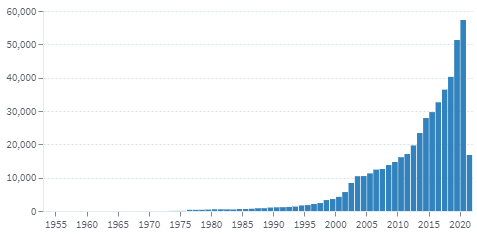
\includegraphics[width=.8\textwidth]{img/patentes/2a.png}
    \end{figure}

    \item Buscar patentes sobre “Fuzzy logic”. Indicar cuántas tiene “Microsoft” sobre esta temática.

    96.435 patentes. 4.696 + 2.141 del conglomerado de empresas de Microsoft.

    \begin{figure}[H]
        \centering
        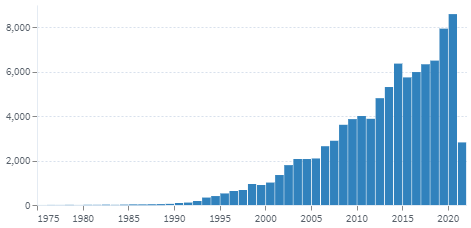
\includegraphics[width=.8\textwidth]{img/patentes/2b.png}
    \end{figure}

    \item Buscar patentes sobre “SVM” (Support Vector Machine). Indicar cuántas tiene “Microsoft” sobre esta temática.
    
    504.121 patentes. 6.829 + 5.415 del conglomerado de empresas de Microsoft.

    \begin{figure}[H]
        \centering
        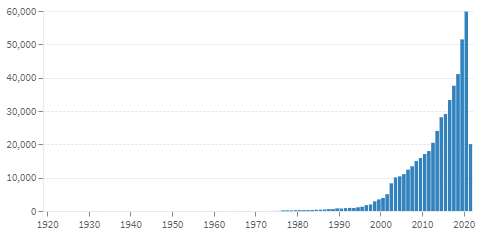
\includegraphics[width=.8\textwidth]{img/patentes/2c.png}
    \end{figure}
\end{itemize}

\subsection{}

Búsqueda de una patente y relación con patentes similares. Por ejemplo con Google Patents o Espacenet.

Buscar la patente WO2020033205A1. Indicar: 
\begin{itemize}
    \item \textbf{Los Inventores}: Stephen Alan Mckinley, David Gealy y Pieter Abbeel.
    \item \textbf{Institución o persona que realiza la solicitud}: Universidad de California.
    \item \textbf{Fecha de la solicitud}: 2019-07-31.
    \item \textbf{Fecha de la publicación}: 2020-02-13.
    \item \textbf{Códigos de Clasificación (CPC)}:
    \begin{itemize}
        \item B25J18/00 (US) 
        \item B25J9/0087 (EP)
        \item B25J9/102 (EP)
        \item B25J9/126 (EP,US)
        \item F16H48/38 (US) 
        \item B25J19/06 (US)
        \item F16H2048/387 (US)
    \end{itemize}
\end{itemize}


% Patentes
% 1) Quizás desarrollar un poco
% 2) Solo el número y (opcional) una gráfica
% 3) Solo las preguntas

% https://worldwide.espacenet.com/patent/search/family/069228268/publication/WO2020033205A1?q=WO2020033205A1 \newpage

% ¿A quíen no le ha dado alguna vez un apretón en la calle? Bueno, no hay forma de evitar que eso ocurra, pero podemos ayudar a hacer el problema más ameno

% ---

% Es necesaria la colaboración extrema y constante de los usuarios para crear la comunidad. Los principios de la app serán difíciles

% Elementos difusos:
% - Urgencia: El usuario podrá elegir entre diferentes niveles de urgencia (inmediato, pronto, cuando sea) que se tendrán en cuenta a la hora de calcular la distancia y los niveles de calidad aceptados.
% - Ubicación: Mediante el geo-localizados del móvil, o incluso la posibilidad de introducirlo a mano si se pretende estimar de antemano


% Información de salida
% - Distancia
% - Tiempo de llegada aproximado
% - Probabilidad de estar ocupado: En base a la cantidad de gente en la zona. Una base de datos adicional (propia o con información introducida por los usuario) podría aportar conocimiento adicional sobre el número de baños, la ubicación (ej: si se encuentra en el bajo de un apartamento es de esperar que aparente haber más gente de la que hay). etc.
% - Nivel de higiene: A partir de las reviews de los usuarios. También se podría hacer un estudio de ciencia de datos recogiendo datos de la ubicación, número de personas, fecha y hora\dots, con el objetivo de predecir el nivel de higiene en ese momento.

% Información de si están rotos
% Ubicación del usuario

% Entre posibles tipos de locales: Restaurantes y cafeterías, universidades, estaciones de tren y bus, edificios públicos, centros comerciales, baños públicos, monumentos, incluso su propia vivienda (para darle mayor prioridad)
% El usuario podría limitar el tipo de sitios en los que acepta a ir, pues por ejemplo sería de mal gusto entrar una cafetería sin consumir nada.

% ---

% Forma de venderlo: Boca a boca
% • Distribución: Dispositivos móviles Android e iOS, en un posible futuro llevado a interfaces web, pero con funcionalidad limitada (no tenemos la ubicación, o se introduce a mano o solo para mirar)
% • Servicio
% • Compra
% • Transporte
% • Formación
% • Garantías

% ¿Por qué mi producto o servicio es mejor?
% • ¿Cómo conseguir que me compren a mí?
% • ¿Cómo puedo sobrevivir a la competencia futura? Los principales competidores serían las aplicaciones de mapas ya existentes (Google maps y el que tenga apple). La única forma de competir con ellas sería contar con un sistema robusto, rápido, preciso, semi-global y con una buena cantidad de soporte por la comunidad de forma que se mantuviera el incentivo en seguir utilizando la aplicación. Si la ellos promovieran la idea a largo plazo no se podría competir, pues sus aplicaciones engloban mayor funcionalidad, son libres de anuncios y tienen mayor prestigio.

    % ==============================================================================

    \setlength{\parskip}{1em}
    \newpage
    % \nocite{*}
    % \bibliography{bibliografia}
  	% \bibliographystyle{plain}
\end{document}